\documentclass[a4paper, 11pt, oneside]{scrartcl}
\usepackage{lpp}
\usepackage{graphicx}
\usepackage{tikz}
\usetikzlibrary{shapes.geometric, arrows}

\begin{document}

\mtitle{Unstructured FEM: Intermediate Report 2}

\mauthor{Mohsin Ali Chaudry, Raghavan Lakshmanan, Abhishek Y. Deshmukh}{A. Emre Ongut}

\maff{SiSc Laboratory}{a.deshmukh@grs-sim.de}{ongut@cats.rwth-aachen.de}

\mabstract{This engineering project of SiSc Lab involves the development of a parallel finite element
solver using unstructured grids. The developed and optimized code is validated using
analytical solutions for a time-dependent engineering heat
transfer problem. This report consists of the approach followed for parallelizing the serial code.
}

\section{Introduction}

\nocite{pp1}
Day by day the requirement for faster computing is increasing owing to increasing complexity and the size of the problems that need to be solved within stipulated amount of time. With advances in hardware hitting the atomic wall, there needs to be a way to use whatever resources are available to the maximum capacity. The large problems need to be solved fast. This motivates the use of the parallel computing that employs multiple cores to solve the problem at hand. However, the serial program needs to be significantly modified if it is to run on multiple cores. In the following sections, the approach followed by us to parallelize the serial code is described.

There are two main computing paradigms \cite{pp1}:
\begin{itemize}
\item Distributed computing
\item Multithreading
\end{itemize}

Distributed computing involves non-uniform memory access. In general, cores and memory are distributed on several machines and are connected through an interconnect. The interconnect may have different topologies like bus, radial, star, torus, omega, etc. depending on the usage. This may or may not require the processors on different machines to communicate the data required to solve the problem being considered. A standard for this communication has been developed and is called MPI (Message Passing Interface) standard.

Multithreading usually involves uniform memory access. All the cores have a shared memory from where they have access to all the data related to the problem being solved. Here, processors don't need to communicate the data. In addition multiple threads can be spawned on each core that can work on different independent piece of data and/or program. A standard for this paradigm is called OpenMP. 

There is also a hybrid paradigm that combines the distributed computing and multithreading. 

The choice of computing model depends upon the hardware available at hand. The RWTH compute cluster supports all of the above computing models. For this project, we have considered distributed computing paradigm because generally clusters with distributed resources are(or may be) readily available to the users. We want our code to be readily usable to maximum possible users who may want to use it for their problem.
\section{Approaches to Parallelizing}
The heat transfer problem to be solved involves a physical domain of interest where the temperature and heat fluxes are to be investigated. The physical domain is discretized into a mesh with triangular elements. Higher the resolution required higher will be the number of mesh elements. In parallel solution, the meshed domain can be divided into parts and each of this part can be distributed to each of the processor for solving. This is known as data parallelism. There are two ways to achieve this. Either read the mesh files namely mxyz and mien parallely or first decompose these files into required number of processors and then each processor can read parallely from its part.

Each of the approaches has its own advantages and drawbacks.

In the first approach (Fig. 1) where processors read parallely from single mxyz and single mien file, each processor may not contain all the data related to node co-ordinates on the same processors. It requires to get missing node information from other processors. This adds the communication overhead. However, there is no need to preprocess the mesh data before running the parallel code. 

In the second approach (Fig. 2), the mesh data is preprocessed. This is done to generate the separate mesh data for each processor so that it has all the elements and node information available. In this case, the serial code needs the least modification. The processors need to communicate the data for the nodes which are common the multiple processors in solver part only. The rest of the parts from serial code can be directly used as they are. This approach is useful because once we have distributed mesh, the same mesh can be reused again and again for parameter studies. It involves one time overhead of generating distributed mesh data. However, this preprocessing takes time for high resolution meshes to be distributed on less number of processors. 

\begin{figure}[!htb]
\centering
\minipage{0.5\textwidth}
\centering
\includegraphics[]{./parallelio_0.png}
\caption{Parallel I/O 1 \cite{llnl}}
\endminipage\hfill
\centering
\minipage{0.5\textwidth}
\centering
\includegraphics[]{./parallelio_1.png}
\caption{Parallel I/O 2 \cite{llnl}}
\endminipage\hfill

\end{figure}

We have followed second approach in our code because once we have a distributed mesh from a preprocessor, the communication overhead is reduced significantly. We can reuse the distributed mesh for further study of the problem using different boundary conditions. We expect good scalability with this approach.

\section{Mesh Partitioning}
Before the mesh can be used efficiently in parallel, another important process has to be performed over it i.e. Mesh partitioning (Fig. 3, 4). Mesh partitioning is a process of dividing the generated mesh into subdomains. These subdomains can be mapped onto a processor of a parallel machine. The primary goal of mesh partitioning is to minimize communication while maintaining load balance. The communication is associated with the nodes that lie on the boundaries between subdomains and are shared by more than one processor. Processors sharing a node must communicate. Communication time depends on both the message sizes, which increase with the number of shared nodes, and the number of messages, which increases with the number of adjacent subdomains. The load can be predicted to be proportional to the number of nodes on that processor. Prediction becomes more difficult when nonlinearities are present. In these cases, the work per node is solution-dependent. 

The partitioners are based on following algorithms:
 Greedy, Kernighan-Lin, Recursive Coordinate Bisection, Recursive Spectral Bisection, Recursive Inertia Partition, Recursive Graph Bisection, algorithm of Miller, Teng, Thurston, and Vavasis, and Simulated Annealingthe. Miller, Teng, Thurston, and Vavasis algorithm uses geometric information to construct a separator, i.e. a set of nodes whose removal separates the mesh into two pieces of roughly equal size. Each of these pieces is then recursively partitioned until the desired number of subdomains is reached. The Miller algorithm, in practice, rapidly produces high quality partitions. 
 
\begin{figure}[!htb]
\centering
\minipage{0.5\textwidth}
\centering
\includegraphics[scale=0.2]{./beforePartition.png}
\caption{Before Mesh partitioning}
\endminipage\hfill
\centering
\minipage{0.5\textwidth}
\centering
\includegraphics[scale=.2]{./afterPartition.png}
\caption{After Mesh partitioning}
\endminipage\hfill

\end{figure}
 
A typical graph partitioning algorithm finds a decomposition of the graph(non-weighted) with preferably the same number of nodes within each partition and with a minimal number of edges between the partitions. 

There are many public mesh partitioning tools. Some of which are listed below:
\begin{enumerate}
\item METIS
\item TOP/DOMDEC
\item HARP
\item CHACO
\item JOSTLE
\item SCOTCH
\end{enumerate}

In this project, a partition utility is used to partition the usual mien FEM connectivity into a set of contiguous subdomains using the Metis graph partitioning library available on cluster. This generates a mprm file which is used in subsequent preprocessing of mesh.

\section{Preprocessor}
The preprocessor takes the raw mxyz, mien, minf, mrng files and decomposes them according to the partitioning defined in mprm file into number of processors specified in "settings.in". This is a serial program. 
It generates an additional file "procb" which contains the information of nodes shared among the processors. This file contains following information per node: global node number, how many processors it is shared with, array of the processor ranks it is shared with. If the node is not shared with any other processor, the array has default value of -1.
Sample procb file for $proc\_0$ is shown below:

\begin{center}

\begin{tabular}{cccccc}

0 & 0 & -1 & -1 & -1 & -1 \\ 

1 & 0 & -1 & -1 & -1 & -1 \\ 

2 & 0 & -1 & -1 & -1 & -1 \\ 

3 & 1 & 1 & -1 & -1 & -1 \\ 

13 & 1 & 1 & -1 & -1 & -1 \\ 

14 & 1 & 1 & -1 & -1 & -1 \\ 
 
15 & 2 & 1 & 2 & -1 & -1 \\ 
 
16 & 2 & 1 & 2 & -1 & -1 \\ 
\end{tabular} 

 \text{Contents of a sample procb file}
\end{center}

% Define the styles for each block
\tikzstyle{startstop} = [rectangle, rounded corners, minimum width=3cm, minimum height=1cm,text centered, draw=black, fill=red!30]
\tikzstyle{io} = [trapezium, trapezium left angle=70, trapezium right angle=110, minimum width=3cm, minimum height=1cm, text centered, draw=black, fill=blue!30]
\tikzstyle{process} = [rectangle, minimum width=3cm, minimum height=1cm, text centered, draw=black, fill=orange!30]
\tikzstyle{decision} = [diamond, minimum width=3cm, minimum height=1cm, text centered, draw=black, fill=green!30]
\tikzstyle{arrow} = [thick,->,>=stealth]
\begin{figure}
\begin{center}
\begin{tikzpicture}[node distance=2cm]

% Nodes
\node (start) [startstop] {Start};

\node (in1) [io, below of=start, minimum width=2cm, minimum height=1cm, text centered, text width=6cm, draw=black, yshift=-0.5cm] {Read: Mesh files: mxyz, mien, minf, mrng, mprm, Input file: settings.in (no. of procs)};

\node (pro1) [process, below of=in1, yshift=-0.5cm] {Define Mesh Structures per processor};

\node (pro2) [process, below of=pro1, minimum width=5cm, minimum height=1cm, text centered, text width=5cm, draw=black] {Distribute the elements and nodes per processor based on partitioning};

\node (pro2z) [process, below of=pro2, minimum width=4cm, minimum height=1cm, text centered, text width=3cm, draw=black] {Generate procb file per processor};

\node (stop) [startstop, below of=pro2z] {Stop};

% Arrows
\draw [arrow] (start) -- (in1);
\draw [arrow] (in1) -- (pro1);
\draw [arrow] (pro1) -- (pro2);
\draw [arrow] (pro2) -- (pro2z);
\draw [arrow] (pro2z) -- (stop);

\end{tikzpicture}\\
\end{center}
\caption{Preprocessor Flow Chart}
\end{figure}

\section{Overall Flow of program}
Overall program flow is shown in figure 5. Each processors runs through the steps shown in the flowchart. This generates VTK data per time step for each processor separately.

%<TikZ code>
\begin{figure}

\begin{center}
\begin{tikzpicture}[node distance=2cm]

% Nodes
\node (start) [startstop] {Start};

\node (in1) [io, below of=start, minimum width=2cm, minimum height=1cm, text centered, text width=6cm, draw=black, yshift=-0.5cm] {Input: Preprocessed Mesh files, Initial and Boundary conditions, Diffusion Coefficient, Source term, No. of iterations, Time step, Data Writing Frequency};

\node (pro1) [process, below of=in1, yshift=-0.5cm] {Define Mesh Structures};
\node (pro2) [process, below of=pro1, minimum width=5cm, minimum height=1cm, text centered, text width=5cm, draw=black] {Calculate Metrics: Jacobian, Element level Matrices};

\node (pro2z) [process, below of=pro2, minimum width=4cm, minimum height=1cm, text centered, text width=3cm, draw=black] {Apply Boundary Conditions};
%\node (dec1) [decision, below of=pro1, yshift=-0.5cm] {Decision 1};

\node (pro2a) [process, below of=pro2z,  minimum width=3cm, minimum height=1cm, text centered, text width=5cm, draw=black] {Solver: Assembly of M and RHS};

\node (pro2aa) [process, below of=pro2a,  minimum width=3cm, minimum height=1cm, text centered, text width=5cm, draw=black] {Solver: MPI Communication of M and RHS for shared nodes among the processors};

\node (pro2ab) [process, below of=pro2aa,  minimum width=3cm, minimum height=1cm, text centered, text width=5cm, draw=black] {Solver: Solve for Temperature [M]\{T\} = \{RHS\}};

\node (pro2b) [io, below of=pro2ab, minimum width=3cm, minimum height=1cm, text centered, text width=2cm, draw=black] {Write VTK Data};

\node (pro2c) [process, right of=pro2b, xshift=2cm] {time+=dt};
\node (dec1) [decision, below of=pro2b, yshift=-0.5cm] {iter<NIter};
%\node (out1) [io, below of=dec1, yshift=-0.5cm, minimum width=3cm, minimum height=1cm, text centered, text width=3cm, draw=black] {Output in Paraview};

\node (stop) [startstop, below of=dec1, yshift=-0.5cm] {Stop};

% Arrows
\draw [arrow] (start) -- (in1);
\draw [arrow] (in1) -- (pro1);
\draw [arrow] (pro1) -- (pro2);
\draw [arrow] (pro2) -- (pro2z);
\draw [arrow] (pro2z) -- (pro2a);
\draw [arrow] (pro2a) -- (pro2aa);
\draw [arrow] (pro2aa) -- (pro2ab);
\draw [arrow] (pro2ab) -- (pro2b);
\draw [arrow] (pro2b) -- (dec1);
\draw [arrow] (dec1) -- node[anchor=east] {no} (stop);
\draw [arrow] (dec1) -| node[anchor=south] {yes} (pro2c);
\draw [arrow] (pro2c) |- (pro2a);
%\draw [arrow] (out1) -- (stop);

\end{tikzpicture}\\
\end{center}
\caption{Overall Program Flow Chart}
\end{figure}


\section{MPI Communication}
Each of the processor reads its portion of mesh, calculates jacobian for each element, assembles element level matrices and finally in solver part assembles the lumped mass matrix (M) and right hand side vector (RHS) of the equation to be solved. However, for the nodes which are shared between different processors, these assembled entities still need the contribution from elements on the other processors. This information needs to be communicated between the concerned processors before the equation can be solved. The procb file which is generated by preprocessor comes into play here. 

Two side communication has been used. The communication is initiated by each of the processors based on the procb file. For the node which is shared between the two processors, the data i.e. M and RHS for the corresponding node is exchanged. On the receiving processor, the addition of received M and RHS to the correct location of existing M and RHS is achieved by matching the global node number.

\section{Results}
\subsection{Validation}
Figures 7 and 8 show the result of the problem with Dirichlet conditions. A rectangular domain is considered for heat diffusion problem. Left and bottom walls are kept at 1000 K while top and right walls are maintained at 300 K and the temperature profiles is allowed to develop over time. The snapshot is taken at t=0.1s. The temperature profiles in both the figures are identical which validates the parallel code.

\begin{figure}[!htb]
\centering
\minipage{0.5\textwidth}
\centering
\includegraphics[scale=0.2]{./serial.png}
\caption{Serial}
\endminipage\hfill
\centering
\minipage{0.5\textwidth}
\centering
\includegraphics[scale=.2]{./parallel.png}
\caption{Parallel: nP=4}
\endminipage\hfill

\end{figure}
\subsection{Scalability}
Figure 9 shows the speedup obtained for finest mesh from Rectangular domain.
\begin{figure}[!htb]
\centering
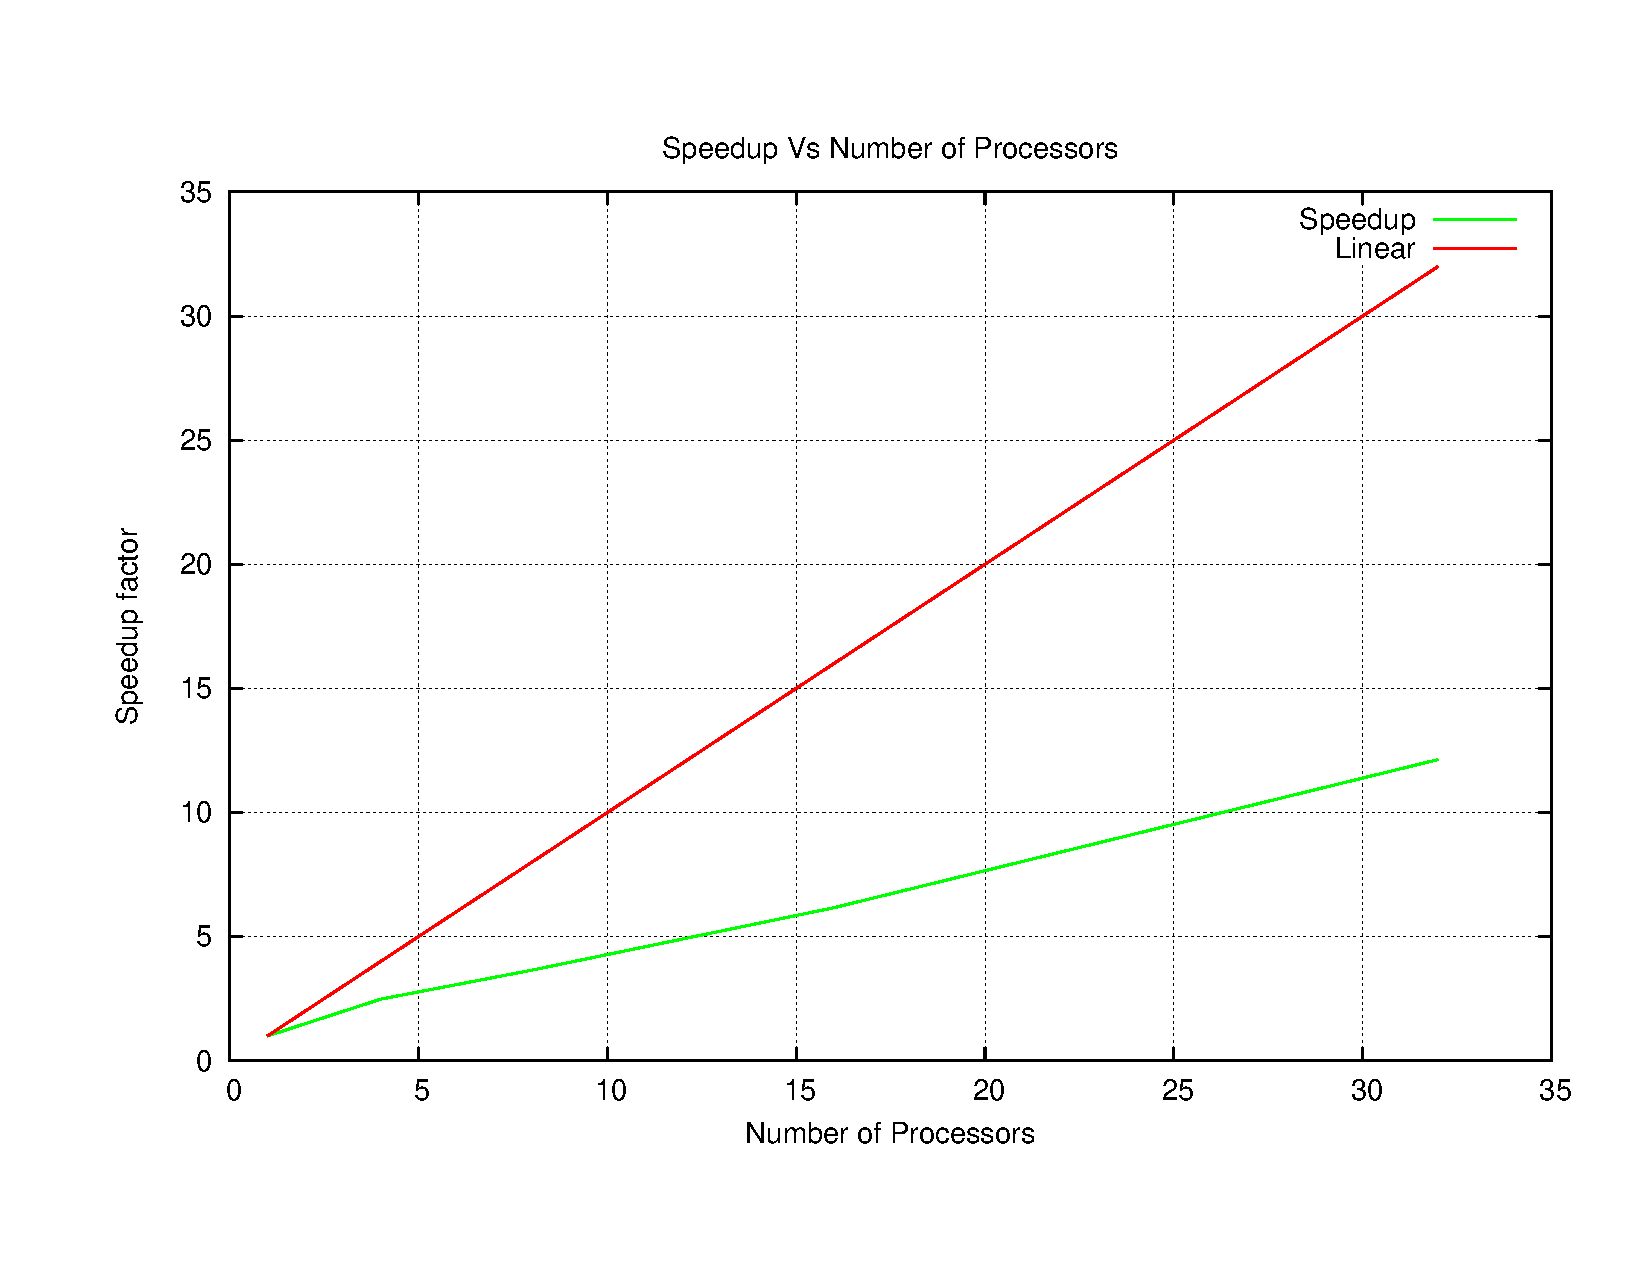
\includegraphics[scale=0.6]{./Timings.pdf}
\caption{Speedup Vs. Number of Processors}
\end{figure}

\section{Summary}
The overall approach of parallelization of a serial code for the problem of interest is to use a distributed computing model. The parallelized code shows some scalability though there is a lot of scope for improvement. The efforts are going on to bring the speedup close to linear one.

\bibliographystyle{unsrt}
\bibliography{literature}

\end{document}
